\documentclass[12pt,letterpaper]{article}
\usepackage{times}
%\usepackage{fullpage}
\linespread{1.66}
\usepackage{lineno}
\usepackage{epsfig}
\usepackage{ulem}
\usepackage{amsmath}
\usepackage{mathrsfs}
\pagestyle{plain}
\linenumbers
%\textwidth 16cm 
%\textheight 21cm
\usepackage[left=1.5in,top=1.25in,right=1.25in,bottom=1.25in,nohead,includefoot]{geometry}

\title{A State Dependent Model for the Development of Life History Skills via Social Interaction}

\author{Nicholas Grunloh (1) and Marc Mangel (2)}
\begin{document}
\maketitle
(1) Program in Statistics and Applied Mathematics and (2) Center for Stock Assessment Research, University of California, Santa Cruz, CA 95064
\section*{Abstract}
Play behavior has been shown to occur  in a surprisingly diverse range of animals, and yet relatively few details are known about the purpose of play in development, or the evolutionary history of play (Burghardt, 2006). %the motivations for its evolution. % of play behavior. 
  This model uses the assumption that social play is an adaptive behavior, as described by Burghardt (2006), to focus on play's contribution toward the development of skill and how this skill development affects an individuals fitness. % fitness  in terms of the fitness gains related to the aquired skill.   
  This model does not focus on any one species directly, but rather takes a general view of play as a fundamental behavior of social animals in general.
  Behavioral models such as this model (SDP) have been shown to be effective tools for inquiry about a diverse range of behaviors by allowing behavioral ecologists to think more deeply about many of the factors contributing toward specific behaviors (Mangel \& Clark, 1988). %about the modivations for modeled behaviors. % for such behaviors.    
  This model suggests patterns of skill development associated with social play and proposes fitness relationships of skill development through time. 

\section{Introduction}
%{\it heading not to appear in final draft}\\

\indent
Five criteria have been identified as consistent features of play behavior (Burghardt, 2006). \\[6pt]
(i) Play is a behavior that is non-essential to the immediate survival of the playing organism.\\[.5pt]
(ii) Play is a self-motivating behavior; done for its own sake, because play is ``fun". \\[.5pt]
(iii) Play differs from any serious version of a similar non-play behavior.\\[.1pt]
\indent (i.e. play can be a non-serious version of other types of behaviors) \\[.5pt]
(iv) Play is heavily repeated (i.e. practiced often), yet loosely stereotyped.\\[.1pt]
\indent (i.e. aspects of play behavior are learned or experimental in nature)\\ [.5pt]
(v) Play only occurs in a stress free environment (a ``relaxed field").\\[.1pt] 
\indent (e.g. an environment with adequate food, that is free of predation or intense competition) \\[6pt]
\indent These criteria do not define play, but they provide a clear framework for the sorts of behaviors that can and cannot be considered play. 
In addition, the above criteria give some sense of just how and when play can occur, for the purpose of guiding a model.  

The evolutionary basis for play behavior is a cloudy topic, but if we consider a few fundamental aspects of play, a structure for thinking about the topic emerges. 
It then becomes clear how to make abstractions in order to formulate a model. 

First imagine behaviors that follow the above criteria (e.g. kittens wrestling).  
From here it is not hard to identify a suite of costs and benefits associated with these play behaviors.   
Caro (1995) identifies several specific costs and benefits to playing in cheetah cubs ({\it Acinonyx jubatus}); see \mbox{Figure 1}.  
In short, the benefits of play can be thought of in terms of the acquisition of skill to be used at some time in the future.
Whether that skill takes the form of maintenance of physical fitness, improved dexterity, or improved social standing, these benefits can be thought of in terms of a single quantity, the player's skill. %survivorship
In a similar way, the costs associated with play can be loosely grouped into manageable quantities.
There are the costs associated with not playing (e.g. not maintaining physical fitness), and there are those costs which occur while playing (e.g. injury and mortality).
%LATER IN DISCUSSION	
%Since a fundamental criterion of play behavior is that play only occurs in a stress free environment, we did not include energy reserves and predation risks in the costs of play. 
%The model assumes a "relaxed field"(Burghardt, 2006), to get at the motivations for play decisions independent of these factors.
%Clearly if these factors became limiting in the model it would disqualify play from occurring by criterion (v) above.

The observation that play occurs in the presence of its costs, suggests that the benefits of play outweigh the costs.
Thus, it is reasonable to assume play behavior has adapted in order to allow individuals the benefits of play, in the face of those costs (Burghardt, 2006).  
Therefore the acquisition of skill through play must be for the sake of the subsequent fitness associated with said skill. 

Assuming play is  adaptive in this way, as opposed to a coincidental non-functional behavior, play decisions must follow some pattern of increasing an organism's fitness through skill (i.e. play occurs because it increases fitness). %Transition to methods, bring inspiration together\\
So even though individuals are driven to play because it is ``fun" the evolutionary theory as to why play has become ``fun", is that play at a given period of development increases an organism's fitness at some time in the future Burghardt (2006); Caro (1988). 
I use Burghardt's criteria for recognizing play behavior as the rules of how and when play are allowed to occur, together with the assumption that play occurs on the basis of increasing (or maximizing) fitness as a foundation for the model.



%LATER
%\noindent-close match-ups maximize skill(self-handicapping)?? slightly higher skills maximize skill per play event?? \\




%\\
%\\
%\includegraphics[width=80mm]{identifyPlay.png}
%\\
%Gordon M.Burghardt:\\
%-ambiguity of play (in general)\\
%-what is play?(outlined criteria)\\
%-social play\\
%-No Stress(ie. NO Predation, NO Energy Reserves)\\
%\\\\
%*****************************************************\\
%-basis for play as adaptive \\
%-lead into discussion of Caro papers with respect to adaptive nature of play\\
%*****************************************************\\
%\\
%\includegraphics[width=80mm]{caro.png}
%\\
%-basic summary of Caro's work and it as inspiration for our model (all 3 papers)\\
%\\
%\includegraphics[width=80mm]{assumtions.png}
%\\
%-Play adaptive\\
%-develops skill\\
%-skill increases fitness\\
%-close match-ups maximize skill(self-handicapping)?? slightly higher skills maximize skill per play event?? \\
%\\\\\\


Methods

  \subsection{\it Overview }
    \indent In order to simplify the dynamics of social play in the model, I consider a focal individual separately from all of the other potential play partners in the environment. % available to play with said focal individual. % enter social play with that focal individual. %We consider a range of focal individual skill levels $i$, as well as a range of potential play partner skill levels $j$. %focuses on the play decisions of a focal individual.
    Individuals can have skill levels ranging from some minimum skill, $S_L$, to some maximum skill, $S_U$. 
    Furthermore, individuals have some skill level at every time within the model as denoted by $S(t)$.
    At any given time, the focal individual may have some particular skill denoted by $i$, and similarly potential play partners have particular skill levels denoted by $j$. %, at any given time period within the model, as denoted by $i$
    Each time period of the model, the skill of the focal individual decrements by, $\alpha$, to capture the idea that skill requires maintenance through repeated practice. %every period of the model to capture the fact skill requires maintenance through practice. that simulate the fact that skill must be maintained by playing   as motivated by skill and the fitness of that skill in the future. %, and if the focal individual decides to play it must pick a play partner.%  whether or not to play,   
    As a focal individual moves through the model's time periods, it makes decisions about whether or not it will play, as motivated by the maintenance of its skill, and the fitness associated with that skill. 
    In order to determine the fitness associated with any given $i$, at a particular time, I first consider the fitness of $i$ for time periods after the periods within the model, as described in Mangel \& Clark (1988) as well as Clark \& Mangel (2000).
    %define T earlier at the number line of life caption
    The function $\phi(i)$ defines the fitness of individuals at the final period of the model, $T$, and for all periods beyond $T$; see Figure 2.
    For particular times within the model, $t$, the fitness associated with any given $i$ is defined by a function, $F(i,t)$, and is related to $\phi(i)$ by the following expression:
    
    \begin{equation}
    F(i,t)=max~E\{\phi(S(T))\}.
    \label{first}
    \end{equation}
    
    %add F(i,T)

    Where $max~E$ refers to the maximum of the expected value of focal individuals terminal fitness based on their skill level at the end of the model.
    Focal individuals maximize their expected future fitness by making play decisions. %; because play is adaptive, focal individuals make play decisions that maximize their long term fitness (i.e. $\phi(S(T))~=~F(S(T),T)~$).
    Thus, $F(i,t)$ is the fitness value associated with the play decisions at $i$ and $t$ that maximizes $F(S(T),T)$. %that maximizes the expected value of the focal individual's terminal fitness.
    $\phi(i)$ and $F(i,t)$ defined in this way, imply that $S(t)$ follows a pattern that maximizes $\phi(S(T))$. %skill after the final time step of the model.%  with the skill level that leads to the maximum expected value of the fitness associated with the focal individual's skill after the final time step of the model.
    This means that organisms behave optimally in the sense that they choose whether or not to play based on maximizing their future fitness, not necessarily their immediate fitness. %in such a way that develops their skill in order to maximize their future fitness.
    By considering focal individuals with a range of skill levels at any given time within the model, I am able to see how factors independent of energy reserves and predation affect an organism's decision to play.   
    
    %The fitness associated with a given skill level at any time, $t$, within the model is determined by a function, $F(i,t)$. % Each skill level is associated with a level of fitness at any time, $t$, within the periods of the model, as determined by a function, $F(i,t)$.
    %Furthermore, each skill level is associated with some level of fitness in the future (i.e. beyond the directly modeled periods) by another function, $\phi(i)$.  %
    %Organisms choose whether or not to play in such a way that develops their skill in order to maximize their future fitness, $\phi(i)$. 
    %As described in (Mangel and Clark, 1988). %$\phi(i)$ is increasing with i so it then means play de %, so each skill levels is associated with some level of fitness at a given time within the model and future fitness beyond the the model. ($\phi(i)$).
    %nd furthermore we can hypothesize about the driving forces of the evolution and adaptation of play. 
    
    %-If the focal individual's fitness at a given time within the model, $F(i,t)$, falls below 
    %\\??include $\alpha$, $\tau$, exit dynamics?? (maybe just a basic idea of whats happening here then in the deep math talk about these details) ??\\    
  
  
    \subsubsection{\it Play Events}
      \indent If it is beneficial for a focal individual to play, and the focal individual is able to find an appropriate play partner, then the focal individual enters a play event with the found play partner. %, and it is beneficial for the focal individual to play, in a given time period of the model, then the focal individual enters a play event.  %  decides to play in a given period of the model, it must pick an appropriate play partner, and enter a play event.% it must pick a play partner.
      I make the assumption that all play partners are willing and available to enter play events with the focal individual, contingent on the focal individual's decision whether or not to play with them. %decides it beneficial for itself to do so. 
      %LATER IN DISCUSSION:
      When a play event occurs between the focal individual, of skill $i$, and a play partner, of skill $j$, the focal individual receives an increment to its skill.
      The increment in skill that the focal individual receives is based on how similar $i$ is to $j$, and the actual increment $i$ receives is determined by a function, $\Delta S(i,j)$. %add inspiration in introduction. %picture of skill difference function regions of significance.     
      In order to capture the idea that skill associated with play events is not necessarily acquired instantaneously, the skill increment, $\Delta S(i,j)$, of a particular play event is awarded to the focal individual a number of time periods, $\tau$, after the play event.  
      Since individuals in the model incur a per period decrement to their skill, $\alpha$, every period of the model, and it takes $\tau$ time periods to gain skill from a play event, it follows that the total decrement to skill of a single play event is $\alpha \tau$. %skill only increases when $\Delta S(i,j)$ is greater than $\alpha \tau$.
      %So the focal individual, of skill $i$, is awarded $\Delta S(i,j)$ skill units, $\tau$ time steps beyond the time period, $t$, of the model in which the play event occurs.
      %Furthermore $i$ loses $\alpha \tau$ skill units while waiting for $\Delta S(i,j)$ to be awarded.
      %The number of time periods beyond the initiation of a play event $\tau$ time periods after the play event at time period, $t$.     
   
      At this point it is worth mentioning that due to the discrete computation of the model, play events occurring when $t$ is near $T$ (see Figure 2) must be truncated so that they are actually shorter than $\tau$ time periods. % handled differently.  
      Note that play events take $\tau$ time periods, thus for some time periods near $T$, $t+\tau$ will be greater than $T$.
      In cases where play events collide with the time horizon of the model, $T$, play events are truncated at $T$.
      If $t'$ is the time period within the model at which a particular play event ends then,
	
	
	~~~~~~~~~~~~~~~~~~~~~~~~~~~~~~~~~~~~~~~~~~~~~if $t+\tau \ge T$ then $t'=T$ \\ 
	\indent ~~~~~~~~~~~~~~~~~~~~~~~~~~~~~~~~~~~~~~~~~~~~~if $t+\tau < T$ then $t'=t+\tau$.
	
	    
      I constructed the model such that $i$ receives the full $\Delta S(i,j)$ for truncated play events, and incurs skill decrements for all of the $\tau$ time periods even though the actual play event may actually be shorter than $\tau$ time periods. % for the periods spent in the play event.
      This keeps the relationship between skill increments and skill decrements for truncated play events consistent with all other time periods of the model. 
      %Thus, play events at the end of the model are particularly valuable, due to discrepancy between the skill increment and the skill decrement. 
    
    \subsubsection{\it Skipping Play Events}
      \indent In some cases it may be more beneficial for the focal individual to skip a play event.
      Skipping a play event in a time period may be because the focal individual is unable to find an appropriate play partner, or because the available play partners in the environment do not allow $\Delta S(i,j)$ to be greater than $\alpha \tau$. 
      If the focal individual decides not to play, then it is not not awarded any skill in the current time and only moves one time period into the future. 
      Consequently, the focal individual only incurs the per period cost to skill, $\alpha$, for a single time period.

    \subsubsection{\it Exiting the Playing Field}
      Caro's(1988, 1995) findings suggest that different types of play occur at differing periods of development (see Figure 1), and thus a model of play behavior must include the ability of playing organisms to stop considering social play as a behavioral option altogether.
      For an individual that has decided to stop considering social play, the pursuit of social play no longer benefits their overall fitness.
      Thus exiting individuals leave the model and would presumably enter another type of play to maintain their skill, or stop playing altogether (i.e. they grow-up); see Figure 2.\\ %The biological interpretation of an individual which exits our model is an individual which has enough skill to ____, and this means that these organisms     
      %If the fitness of a focal individual at any time of the model, $F(i,t)$ ever falls below their future fitness, $\phi(i)$, then the focal individual is allowed to stop perusing play partners and is said to exit the model.

\begin{table}[h]
\caption{Relavent model parameters, variables, and functions.}
\centering
\begin{tabular}{l l}
\hline
$S(t)$ & Meaning \\ 
\hline 
$i$ & focal individual's skill \\ 
\\
$j$ & play partner's skill \\
\hline 
Parameters & Meaning \\
\hline
$\alpha$ & per period cost to skill\\
\\
$\tau$ & time required to play \\
\hline
Functions & Meaning \\
\hline
$\lambda_j(t)$ & probability that the focal individual encounters \\ 
$ $ & a play partner of skill $j$\\
\\
$\Delta S(i,j)$ & focal indviduals increment in skill as a result of \\ 
$ $ & playing with a partner of skill $j$\\
\\
$F(i,t)$ & fitness of the focal individual, with skill $i$ at \\
$ $ & some time $t$, within the modeled period \\
\\
$\phi(i)$ & future fitness of the focal individual, with skill $i$, \\
$ $ &  for periods after the final period of the model\\
\\
$D^*(i,j,t)$ & an array of play decisions for the focal individual \\
$ $ & encountering a play partner at some time period of model \\ 

%Pr(focal individual encounters a play partner of skill $j$)
\hline
\end{tabular}

\label{Tab:param}
\end{table}
    %As a discrete model we can only consider some range of time to consider play behavior.
    %Similarly we can only model a range of skill levels.
    %This is not worrisome, considering that individuals only display social play for a limited window in their development anyhow.
    %We define $T$ to be the final time period of the model and $t$ to be any other specific time period within the model.
    %Furthermore, the model only considers play behavior between a lower limit of skill, $S_L$, and an upper limit of skill, $S_U$. 
        
    \subsubsection{\it Skill Increment Function}
      In order to explain the way that a focal individual develops its skill within the model I must determine the amount of skill that any focal individual will get from a particular play event.
      As described in section 2.1.1, the skill increment is based on how similar $i$ is to $j$.
      The more similar that $i$ is to $j$ the greater that $\Delta S(i,j)$ should be, in general.
      This property comes from the acknowledgment that individuals of similar skills are likely to be developing similar aspects of their overall skill suite (Burghardt, 2006).
      $\Delta S(i,j)$ reaches a maximum, defined by $S_{max}$, when $i=j$, and as $i$ becomes more different form $j$, $\Delta S(i,j)$ decreases.
      For the computation of my general model, I use a Gaussian function for $\Delta S(i,j)$, although in reality the specific attributes of this this function may be changed to better fit the particular life history and social structure of a particular model organism.% may differ   is defined by the following Gaussian function:    
      
      \begin{equation}
      \Delta S(i,j) = \Delta S_{max} e^{ - \left( (i-j)^2 \over 2\sigma^2 \right) }.
      \label{sdf}
      \end{equation}
      
      Here $\sigma$ is a parameter that describes how similar the focal individual must be to the play partner in order to receive a meaningful skill increment from a play event; see Figure 3.
      Biologically, a skill increment of $S_{max}$ is only possible in a ``perfect" play event where $j$ is perfectly suited for playing with $i$.
      Therefore $\Delta S(i,j)$ will always be maximized when the focal individual and the play partner have the same skill (i.e. $i = j$).    
      Notice that the symmetry of Eq.(2) means that $\Delta S(i,j)$ does not really depend on either $i$ or $j$, but rather the absolute difference between $i$ and $j$.    
      
      As a thought experiment to help understand how focal individuals are motivated by the acquisition of skill through $\Delta S(i,j)$, consider a focal individual that makes play decisions based only on the effects of those behaviors in the next time period.
      This myopic focal individual does not care about any of the opportunity costs of playing with one play partner over a better suited play partner. 
      The myopic focal individual only considers whether a play partner ultimately causes an increase or decrease in skill, regardless of any ill effects these decisions my cause in further time periods. 
      For the myopic focal individual the decision to play, or not, is really just a comparison between the skill decrement of the play event, $\alpha \tau$, and the skill increment, $\Delta S(i,j)$, see Figure 3.
      If $\Delta S(i,j)$ is greater than $\alpha \tau$ then the myopic individual will always play regardless of how small the difference, and if $\alpha \tau$ is the greater than $\Delta S(i,j)$, the myopic individual with never play.   
      This is how optimal behavior focal individuals, with only a single time period remaining in the model, behave due to the lack of opportunity costs at $t=T-1$. % remaing will behave due to  in this model behave when there is only a single time period remaining in the model, because they 
      However as $t$ approaches $1$ from $T$ we will see how the optimal focal individual considers factors that introduce opportunity costs and lead to more selective behavior than in the myopic case.   
          
    \subsubsection{\it Play Partners}
      As seen in $\Delta S(i,j)$, the skill increment associated with a play event is in some sense dependent on $j$. 
      We will see other ways that $j$ affects the play decisions of the focal individual. 
      Namely, the focal individual does not only consider how choosing a particular play partner affects $\Delta S(i,j)$, but also the probability of encountering each $j$. % hae to deal with must not only deal with the actual play event with      
      Thus I need to declare a distribution for the skill levels of all the potential play partners in the environment.
      By doing so I bring the skill structure of the environment into the model.
      In order to accomplish this I consider $\lambda_j(t)$ as the following probability,  %If $lambda_j(t)$ is the probability of a random observer encountering a play partner, of a particular skill level $j$, at the time of interest, then it is reasonable to state 
      
      \begin{equation}
      \lambda_j(t)=Pr(focal~ individual~ encounters~ a~ potential~ play~ partner~ of~ skill~ j~ at~ t).
      \end{equation} 
      %LATER DISCUSSION: encountering more than one play partner at a time. 
      
      A probability of encountering a play partner of any given skill level in the environment adds important considerations into the focal individual's decision to play.
      This distribution allows the focal individual to make play decisions based, not only on the fitness associated with their skill, but also the likelihood of maintaining that skill through play. %  consider the itness bring the skill structure of the environment into our model.
      %It turns out that this consideration has large implications on the focal individual's decision to exit play behavior altogether. 
      The specific hypothetical environment of my general model is defined by the following exponential probability density function:       
      
      \begin{equation}
      \lambda_j(t) = \delta_n e^{-cj}.
      \label{lambda_j}
      \end{equation}
      
      Where, $c$ is a scale parameter characterizing how quickly members of the potential play partner population leave the play environment.
      $\delta_n$ is a normalization constant chosen so that \\$\sum_j \lambda_j(t)~\le~1$, and thus the remaining  probability is tied up in events where the focal individual cannot find any play partner, $(1-\sum_j \lambda_j(t)~)$. %inorder to conserve probability, the remaining $(1-\sum_j \lambda_j(t)~)$ is the probability of not encountering any play partner.
      %This allows for the possibility that the focal individual may not encounter any play partner in a given time period, with probability $(1-\sum \lambda_j(t)~)$.
      The distribution of the potential social play partners in the environment, as an exponential, translates into an environment with initially many low skill individuals.
      As potential play partners develop, and leave the population, a decreasing number of high skill individuals are left in the population. %as potential play partners develop and leave the pool of potential play partners. 
      
      
    \subsubsection{\it Fitness Functions}
      %As a basis for thinking about the fitness of a focal individual, let us start by considering the fitness of an individual at the end of the model, $\phi(i)$. 
      %The function $\phi(i)$ must account for all of the fitness associated with an individual of skill $i$ at the end of the model, and for the rest of the individual's life as described in Mangel and Clark (1988). 
      %Eq.(\ref{first}) shows that $F(i,t)$ is based on the terminal fitness function $\phi(i)$.
      %In order to use this logic I must first have some idea about the features $\phi(i)$ should have.
      As individuals gain skill, it is intuitive that their fitness will increase, thus I assume that $\phi(i)$ will be some sort of increasing function.     
      Specifically, I choose a logistic function that has some threshold skill level at which organisms quickly develop fitness, as they would in adolescence (see Figure 4).   
      
      \begin{equation}
      \phi(i) = {(i-S_L)^\gamma \over {(i-S_L)^\gamma+(S_o-S_L)^\gamma} }.
      \label{phi}
      \end{equation}
      
      Where $S_o$ is the skill at which half maximal fitness is achieved, and defines where the skill threshold of adolescence will occur.   
      In Eq.(5), $\gamma$ is a steepness parameter of $\phi(i)$ that defines how quickly fitness increases with increased skill near the skill threshold
      
      \begin{equation}
      F(i,T) = \phi(i).
      \label{equivalence}
      \end{equation}
      
      That is, focal individuals behave in such a way that maximizes the expectation of their fitness at the end of the model, not necessarily their fitness in the next time step.
      Eq.(\ref{first}) makes use of the assumption that play behavior is adaptive, and thus play decisions maximize the focal individual's fitness.
      This means that by making a reasonable prediction of the fitness of the focal individuals for time periods beyond the model, $\phi(i)$, I can work backward, from $T$, in order to determine the fitness of individuals at every time within the model.   
      
    \subsubsection{\it Stochastic Dynamic Programming Equation (SDPE)}
      %At this point we have established all of the components necessary for a focal individual to make decisions about whether or not to play at a given time within the model.
      
      %ABOVE
      %As established previously, individuals decide to play based on maximizing the expectation of their future fitness, $\phi(i)$, and they take values of $F(i,t)$ that are based on maximizing their position on that terminal fitness function.
      For times prior to the the time horizon, $T$, I consider a weighted average of all of the possible optimal decision fitness values that the focal individual can take, from $t$ to the next time period \mbox{($\displaystyle\operatorname*{t+1}_{skip}$ or $\displaystyle\operatorname*{t+\tau}_{play}$)}, based on the probability $\lambda_j(t)$  of encountering each of the potential play partners at $t$. % occurring, $\lambda_j$. %of encountering the play partners which. %the fitness of the focal individual associated with all of the possible situations that the individual might encounter in making the decision to either enter a play event, skip a play event, or exit the playing field in the previous time period
      This weighted average is dynamic in the sense that the average is calculated differently based on the decisions associated with each possible potential play partner.
      Let us start by considering the DPE for the simplified situation where the focal individual must only decide whether or not to play.
      Thus, the focal individual is ensured not to exit the model in the following equation. % organisms that stay within the model and then must decide whether or not to play in the given time 

      \begin{equation*}
      V_{cont}(i,t)=\bigl(1-\sum_j \lambda_j(t) \bigr) ~F(i-\alpha,~t+1) ~+~ \sum_j \lambda_j(t)~max
      \begin{cases}
	F\bigl(~ i + \Delta S(i,j) - \alpha \tau,~t+\tau ~\bigr)                                & D^*(i,j,t)=1 \\
	F(i-\alpha,~t+1) 				                              & D^*(i,j,t)=0
      \end{cases}. 
      \end{equation*}

      %Above $\lambda_{null}$ is the probability of not encountering any play partner, while each $\lambda_j$ is the probability of encountering play partners of each skill level.
      %Each possible play encounter is associated with a fitness based on the skill level, $j$, of the play partner encountered.
      Above, $max$ refers to the the maximum value between the fitness' associated with playing with $j$ or skipping a play event with $j$.
      For example if the focal individual does not encounter a play partner it is not awarded any skill, but does incur the per period cost to skill, $\alpha$, for one period of the model. 
      So the fitness associated with this situation is $F(i-\alpha,~t+1)$ with probability $\bigl(1-\sum_j \lambda_{j}(t) \bigr)$.     %  a so the fitness value associated with not encountering a play partner is the fitness assciated with   that  %Eq. (\ref{Fmax})  
      However, the focal individual may find a play partner of any of the available skills with probability $\lambda_j(t)$.  
      In these cases the focal individual must decide between entering or skipping a play event with the encountered play partner of skill $j$. 
      If the focal individual decides to play with a given play partner it is awarded the skill increment for playing with that play partner, $\Delta S(i,j)$, and a skill decrement, $\alpha$, for every period of the play event.
      Since play events take $\tau$ time periods, the total decrement that $i$ receives is $\alpha \tau$, and this makes the fitness associated with playing $F\bigl(~ i + \Delta S(i,j) - \alpha \tau,~t+\tau ~\bigr)$.
      Of course, if $\Delta S(i,j)$ does not overcome $\alpha \tau$ it will not be any more beneficial for the focal individual to play with $j$, than to skip a play event.
      Thus the fitness associated with skipping a play event is $F(i-\alpha,~t+1)$.
      The amount of time required to skip playing does not involve entering a play event, so the time increment is only one period. % only takes $\tau$ time steps
      In order to anaylze the resulting play decisions of $V_{cont}(i,t$, play decisions are stored in an array, $D^*(i,j,t)$.
      When the focal individual encounters a play partner it either chooses to enter a play event, $D^*(i,j,t)=1$  or skip a play event, $D^*(i,j,t)=0$, based on which of the two fitnesses are higher. 

      %LATER MORTALITY IN DISCUSSION
      In addition to choosing whether to play or skip in each time period, the focal individual must consider if it still wants to pursue social play behavior altogether. %wheter or not it is still worth it to them model forces focal individuals to make descions about exiting the pursuit of play altogethor or staying in the model
      %It does so based on the % same way that focal individuals decide whether to play or skip with a given play partner, by choosing the option which maximizes their fitness.
      Focal individuals decide to continue in the model or exit the model based on the decision that again, maximizes their future fitness.
      
      \begin{equation}
      F(i,t)=max
      \begin{cases}
      V_{cont}(i,t)                                                                   & cont_{_i} \\
      \phi(i)                                                                         & exit_{_i}
      \end{cases}
      \label{breif}
      \end{equation}
      
      %$F_{stay}$ is calculated as seen in Eq.(\ref{Fmax}) and it itself involves making the decision of whether or not to enter or skip a play event at any time, with each play partner.
      %$F_{stay}$ is first caluculated in the manner that maximizes itself.
      %$F_{stay}$ is then compared whith $\phi(i)$ and the maximum fitness value between the two is then the fitness associated with the decision of the focal individual. 
      %If $\phi(i)$ is the greatest fitness value then the focal individual leaves the model, but if $F_{stay}$ is the greatest fitness value then the focal individual still considers engaiging in social play.
      %Keep in mind that $F_{stay}$ is itself calculated based on the average of decisions to play with each potential play partner of skill $j$. % either enters or skips a play event .
      %The full SDP used in the model can then be written as 
          

      %\\\\
      %full crazyness sdp
      %\begin{equation}
      %F(i,t)=max
      %\begin{cases}
      %\lambda_{null} ~F(i-\alpha,~t+1) + \sum_j \lambda_j ~ max
      %\begin{cases}
	%F(~ i + \Delta S(i,j) - \alpha \tau,~t+\tau ~)   \\    
	%F(i-\alpha,~t+1)                                       
      %\end{cases}                                                                    & \begin{array}{1} play\\ skip \end{array}   \\                                           %dbinom{play}{skip}\\%^{play}_{skip}
      %\phi(i)                                                                        & ~~exit.
      %\end{cases}
      %\label{bigDaddy}
      %\end{equation}

      Eq.(\ref{breif}) incorporates all the decisions a focal individual must make, and it is solved backwards in time from the terminal condition.
      Every time period of the model $V_{cont}(i,t)$ is solved and compared with $\phi(i)$, as in Eq.(\ref{breif}).
      Solving the SDPE in this way yields the optimal behavior fitness values associated with focal individuals of every possible skill level $i$, considering play partners of every possible skill $j$ on the interval $[S_L,S_U]$, at every time within the model (i.e. $F(i,t)$ ).
      In addition to $F(i,t)$, the SDPE also yields the optimal decision array $D^*(i,j,t)$ containing the associated play decisions (i.e. play, skip, or exit) for the focal individual at every combination of $i$, $j$, and $t$.  

%      \begin{equation}

%	F(i,t)=
%	\begin{cases}
%	\lambda_{null} F(i-\alpha,~t+1) + \sum_j \lambda_j ~ max
%	\begin{cases}
%	  F(~ i + \Delta S(i,j) - \alpha \tau,~t+\tau ~)  \\
%	  F(i-\alpha,~t+1)
%	\end{cases} & F(i,t)>\phi(i) \\
%	\phi(i)     & F(i,t) \le \phi(i)

%	\end{cases}
%      \end{equation}
      
    \subsubsection{\it Monte Carlo Implementation of Play Decisions Forward in Time}  
      To predict the behaviors of individuals, I use $D^*(i,j,t)$ to run a Monte Carlo model forward through time. 
      The Monte Carlo forward iteration simulates a number of focal individuals, $k$, making optimal play decisions as predicted by Eq.(\ref{breif}), through the modeled period of time. 
      Initially $k$ focal individuals are generated with uniformly drawn random skill levels on the interval $[S_L,S_U]$. 
      In each time period of the simulation, each of the $k$ focal individuals encounter a potential play partner drawn randomly from the probability distribution of encountering potential play partners of skill $j$, Eq.(\ref{lambda_j}). 
      At each potential play encounter the focal individual either enters a play event, skips a play event, or exits the model based on the predictions generated by Eq.(\ref{breif}), at the particular $i$, $j$, $t$ conditions of the given play encounter.  
      The model follows the following algorithm for each of the $k$ focal individuals:
      \\
      (1) $t=0$\\
      (2) Draw a random uniform focal individual skill level, $I_k(t)$, on the interval $[S_L,S_U]$.   \\
      (3) Draw a random potential play partner skill level, $J$, from Eq.(\ref{lambda_j}).\\
      (4) Look up the appropriate play decision, $D^*(I_k(t),J,t)$.\\ 
      (5.1) If the play decision is play; $I_k(t+\tau)=I_{k}(t)+\Delta S(I_k(t),J)-\alpha \tau$ and $t \rightarrow t+\tau$.\\ 
      (5.2) If the play decision is skip; $I_k(t+1)=I_{k}(t)-\alpha$ and $t \rightarrow t+1$.\\
      (5.3) If the play decision is exit; $I_k(t+1)=I_{k}(t)$ and $t \rightarrow T$.\\
      (6.1) If $t < T$ go to step (3). \\
      (6.2) If $t \ge T$ then $I_k(T)=I_k(t)$.   

  
%  \subsection{\it Basic Model}
%    -functions description
%    \subsubsection*{\it predicting decisions backward from T}
%    -backward iterative method (Mangel & Clark, 2006)
%    -flow(code appendix)
%    -evaluate for every skill 
%    -every possibility to tell forward iteration when to play and not 
%    \subsubsection*{\it simulating behavior forward in time}
%    -Dynamics of Skill(how to get skill and lose it/its connection to fitness)\\
%    -Choosing a play partner(threshold of play/Skill difference function)\\
%    -Skill Distribution of Environment(static/dynamic)\\
%    -Terminal Fitness(basis of SDP)

%    \subsubsection*{\it adding mortality}
%      -modification to DPE\\

%  \subsection*{\it Dynamic Environment Model}
%    \includegraphics[width=80mm]{parameters.png}\\
%    
%    \includegraphics[width=70mm]{esd.png}\includegraphics[width=70mm]{sdfIntroThinking.png}\\
%    -environment skill distribution\\
%    -skill difference function\\
%    -future fitness function(logistic)

%    \subsubsection*{\it exit model}
%      \includegraphics[width=80mm]{exitDPE.png}

%    \subsubsection*{\it exit model w/ mortalitiy}

%  \subsection*{\it Forward}
%    -Monte Carlo Simulation
%    -environmental skill distribution constant v. dynamic????
    
%    \subsubsection*{\it exit model}
%    -taking play decisions for i,j encounters from exit model
    
%    \subsubsection*{\it exit model w/ mortalitiy}
%    -working on it


\section{Results}
  \subsection{\it SDP}
    Fully solving Eq.(\ref{breif}) backwards in time yields two primary results.
    Firstly, I obtain the play decisions for every $i$, $j$, and $t$ combination from $D^*(i,j,t)$, and secondly, I obtain the fitness values for every focal individual's skill level and time, $F(i,t)$. 
    
    \subsubsection{\it Play Decisions}
      $D^*(i,j,t)$ shows that focal individuals choose to play with a range of similarly skilled individuals about the diagonal of $D^*(i,j,t)$ where $i=j$.
      This is not surprising considering the shape of $\Delta S(i,j)$ and its symmetry about $\Delta S_{max}$ at $i=j$.
      If the cost of play, $\alpha \tau$, ever becomes much larger than, $\Delta S(i,j)$, a focal individual will not choose to play with them.
      Thus, $\alpha \tau$ is a major driver in determining the extent to which $i$ must be similar to $j$ in order for the focal individual to enter a play event. 
     
      I see patterns in the total range of playable $j$'s based on the focal individuals skill and the time period of the model in which a play event occurs. %that at any given time, as $i$ increases the total span of playable $j$'s increase.       In addition to play events only occurring in a range about the diagonal of $D^*(i,j,t)$ where $i=j$, 
      That is to say that at some $t$ and $i$, there exists a maximum $j$ that is beneficial for $i$ to play with; I will call this maximum playable $j$, $\hat J_{i}$.
      Similarly there is some minimum $j$ that is beneficial for $i$ to play with, denoted by $\check J_{i}$.
      Consider the following statistic as a representation of the total range of potential play partners for every combination of $i$ and $t$ shown in Figure 5.
      
      \begin{equation}
      R(i,t)=\hat J_i - \check J_{i}.
      \end{equation}
      
      %R(i|t)
      holding $t$ constant, in general as $i$ increases $R(i|t)$ increases, until a threshold $i$ for which every subsequent $i$ exits the model.
      Biologically this means that as individuals gain skill, they are willing to play with a broadening range of individuals in the environment.
      Pre-exit high skill individuals have incentive to broaden their play range because they do not need much more fitness in order to exit the model.
      These individuals can get the skill that they need to exit the model from a wide range of $j$'s.
      However, low skill individuals need to increase their fitness a lot, and need large values for $\Delta S(i,j)$ to get high fitness.
      Thus, at all values of $t$, low skill individuals are very selective for play partners, such that $\hat J_i \approx i$ and $\check J_i \approx i$. 
      
      %R(t|i)
      Holding $i$ constant in general as $t$ increases $R(t|i)$ also increases.
      This is due to the fact that as individuals approach the time horizon they behave more and more similarly to the myopic focal individual discussed in section 2.2.1. % desperate for fitness, so they are forced to accept lower and lower values of $\Delta S(i,j)$.
      Although optimal focal individuals do behave similarly to the myopic focal individual when $t$ is near $T$, the only time optimal focal individuals truly behave myopically is when $t=T-1$.   

      Additionally as $t$ increases, the exit threshold occurs at decreasing values of $i$. % changes because of $F(i,t)$ increases with time.
      This is caused by the dynamics of $F(i,t)$ with time as seen in Figure 6.
      When many time periods remain in the model, $F(i,t)$ is greater than $\phi(i)$ for most values of $i$, excluding a few exit skills.
      So most values of $i$ consider play behavior for some period of the model.
      As $t$ approaches $T$, $F(i,t)$ decreases to approach $\phi(i)$ and thus $F(i,t)$ falls below $\phi(i)$ at lower values of $i$ at later time periods of the model. 
         
      % are more willing to play with %they enter a positive feedback loop
         
      
      
      %-lead to heatmap
      
      %Another factor in determining the range of beneficial play events is $F(t+\tau)$ (in the case of a play event) as compared with $F(t+1)$, in the case of a skipped play event.
      %The slope of these two function determines just how big a fitness increase is associated with any change in skill from i in each respective case.
      %In places along these curves where the slope is steep  
      %$\alpha \tau$ together with the shape of $\phi(i)$ determine the range of possible play partners that are beneficial to play with.
      
      % the similarity 
      %Considering that $\Delta S(i,j)$ is a symmetric function about its maximum, and that is is only possible for a focal individual to play
      %-only play if $\Delta S(i,j)$ greater than $\alpha \tau$

    \subsubsection{\it Fitness}      
      As seen in Figure 6, when $t$ is less than $T$; $F(i,t) \ge F(i,T)$.
      This is due to the amount of time left in the model at $t$.
      Notice that when many time periods of the model remain $F(i,t)$ is greater than $\phi(i)$. %initially for low skill individuals $F(i,1)$ is much greater than $F(i,T)$.
      When there is a lot of time left in the model, individuals with relatively low skill can have high fitness due to the prospect of gaining skill in the future.    
      Also notice when individuals gain high skill they exit the model at the skill level where $F(i,t)$ converges with $\phi(i)$.
      So as $t$ approaches $T$, $F(i,t)$ approaches $\phi(i)$ from the top, and this exit skill decreases.


      %When individuals gain high skill they exit the model at the skill level where $F(i,t)$ converges with $F(i,T)$. 
      
      %As $i$ increases, $F(i,1)$ ap 
       %  a relatively flat line for low skills, and it is only at high skill with Since $F(i,t)$ is based on $F(i,T)=\phi(i)$ 
      
      
      %\includegraphics[width=80mm]{exitResults.png}\includegraphics[width=80mm]{backBig.png}\\
      %-initially at low skill fitness is higher than later time periods \\
      %-Staying at low skill decreases fitness(static scenario, obvious)\\
      %-removes low fitness(below future) @ high skill, low time.(looks like it just truncates fitness below future fitness, this increases low skill fitness. why? )\\
      %-high fitness @ low skill, low time: the prospect for gaining more skill in the future\\% because usually initial fitness is higher than future fitness for all skills, but because of ________  (a crucial time) 
      %-initially orgs have the highest fitness, and exit at high skill.\\
      %-as time proceeds fitness decreases and exit skill lowers\\
      %-with increased T initial fitness increases to higher levels.(primarily in exit model, in basic model fitness hardly increases )\\
      %-so only very high (basically max) skills exit, as T increase initial exit skill increases.\\  
      %(maybe some of this stuff belongs in discussion?)
  \subsection{\it Monte Carlo Simulation}
    Using $D^*(i,j,t)$ to run a Monte Carlo Simulation, there are many aspects of play behavior that can be considered.
    Specifically I am interested in the long term perspective of play and how an individual's skill affects long term play decisions.      
    \subsubsection{\it Initial \& Final Skills}
      Initial skills are uniformly distributed, so by considering the distribution of the final skills I can see the effect of play behavior on the population.
      Figure \ref{Fmcmc} shows the final skill distribution of $k=250$ individuals making optimal decisions for 40 periods of the model.
      This distribution appears to be bimodal, and if $k$ is increased, the final skill distribution becomes a clear bimodal distribution.
      The mode centered around skill 30 is representative of the accumulation of all exiting individuals throughout the modeled periods. 
      The mode centered around skill 15 is the most common skill for individuals who have not exited the model yet.
      
      Figure \ref{Fmcmc} can be extended into the scatter plot seen in Figure \ref{mcmc} to see the relationship between the initial skill of the $k$ simulated individuals. 
      The dotted red one-to-one line on Figure \ref{mcmc} shows the final skill level required to maintain the initial skill level the individual entered the simulation at.
      Considering individuals enter the model with a uniform distribution over the range of possible skills, This ensures that the simulation will show all of the possible play strategies in the environment.    
      It is immediately noticeable that some organisms start with high enough skill to exit the model immediately.
      These are the individuals with initially high skill, on the one-to-one line in the region labeled ``Exit".
      Organisms with initial skills below the initial exit skill all want to play to some degree, but the lower the initial skill the more selective the play decisions become due to the large amount of skill they need to gain.
      The lower the skill of the organism, the more selective the organisms is in choosing a play partner, however $\lambda_j(t)$ is defined such that these low skill individuals have a high likelihood of encountering just the play partners that they seek.
      Playing organisms that have high enough final skills to find themselves above the one-to-one line, in the region labeled ``Lucky" are individuals that were able to successfully find the play partners that they need to improve their skill from their initial state.
      Playing organisms that end up below the one-to-one line, in the region labeled ``Unlucky" are individuals want to play, but were not able to find the play partners that they need to improve their skill. %  enough initially, but cannot find any favorable play partners purely due to chance, and thus end up in the region labeled ``unlucky". % were not lucky enough to find the play partners they need to improve their skill from their initial state. 
      For low skill individuals it is relatively easy to find appropriate play partners, and thus they most often end up in the ``Lucky" region.
      

    %\subsubsection{\it Skill Progressions \& Mortality}\\
      
    \section{Discussion}
  \subsection{\it The Relaxed Field}
    Since a fundamental criterion of play behavior is that play only occurs in a stress free environment, we did not include energy reserves or predation risks into the costs of play. 
    This model assumes a ``relaxed field"(Burghardt, 2006), to get at the motivations for play decisions independent of these factors.
    Clearly if these factors became limiting in the model it would disqualify play from occurring by Criterion v listed in Section 1.

    This model can be modified relatively easily in-order to consider play behavior with respect to these factors, but as a starting point it is instructive to understand the basics of play behavior within this simple model first.
    As more intricate models are made on play behavior, added considerations may make it hard to see some of the basic forces driving play behavior as seen in this model.

  \subsection{\it $D^*(i,j,t)$ Exception Pocket}
      %T_{play} exceptions of D*(i,j,t)
      Looking at Figure \ref{mapExit}, we can see that the patterns outlined in Section 3.1.1 do hold true in general, however there is a pocket of time and skill where these patterns do not hold true.
      I propose that this can be explained by the finite time horizon of the model, and its relation to play events as defined by the model. 
      Recall that for time periods near $T$, play events cause $t+\tau$ to be greater than $T$; see Section 2.1.1.   
      Due to the construction of the model the skill increments and decrements for play events in these periods are consistent with all other time periods of the model, however the fitness values associated with these skill levels must be truncated at $F(i,T)=\phi(i)$ because by definition fitnesses for time periods beyond $T$ are defined by $\phi(i)$. %this makes play events at the end of the model particularly valuable, due to discrepancy between the skill increment and the skill decrement.
      %This means that individuals needing a lot of skill at the end of the model have a pocket of time in order to make larger than normal skill jumps.
      %This also means that low skill individuals do not want to waste any time periods of this pocket by entering the pocket already in a play event.
      This has the effect of decreasing $R(i,t)$ for time periods just prior to the final time periods of the model.
      Skills high enough to exit the model have lower than expected values for $R(i,t)$ several time periods before these individuals exit the model.  % levelstime periods just before the beneficial pocket, so that individuals finish any previous play events, prior to entering the pocket.
      %Thus individuals are available to enter play events once inside the pocket.
      Individuals several time steps before the end of the model are very selective in their choice of play partners because the fitness associated with any skill level in these time periods of the model has been truncated to $F(i,T)=\phi(i)$. %are appraised to have an artificially low value as a product of the time truncation of play events. %in this period of the model. % want to maximize their skill increment.
      This seems to be one of the major challenges of this model since real play is not actually bounded in this way. 
      For this reason it is useful to run the model with large values of $T$ and consider the general trends of the model prior to this exception pocket. 
      
      %Again in general, I find that low skill individuals will be relatively selective in their play decisions, looking to play primarily with other low skill individuals of similar skills.
      %As skill becomes high, individuals are more willing to play with individuals of very dissimilar skill levels. 
      
      %handicap
      %These high skill individuals have incentive to self-handicap, due to the relative abundance of each type of potential play partner.
      %In the model there are relatively few high skill individuals in the model, but there are many low skill individuals to play with.
      %The high abundance of low skilled potential play partners helps motivate high skilled individuals to play with then due to there high probability of encounter, as defined by $\lambda_j(t)$ in Eq.(4).  
      %Although low skill individuals do not offer a lot of skill benefit to high skill individuals, the skill benefit that they can offer to high skill individuals is just enough push them over the exit threshold of the model. % just enough skill benefit for high skill individuals 
      
      %High skill individuals do not display this behavior because they will easily exit the model with many play partners no matter when they play with them.  
      %Since real individuals presumably would not have a finite time horizon I propose that $R(i,t)$ is artificially high for low skill individuals at times immediately before the pocket, and artificially low at times within the pocket. 
      %At this point it is worth mentioning that the fact that the model is discrete causes later time period play events to be shorter than $\tau$ time periods. % handled differently.  
      %Note that play events take $\tau$ time periods, thus for time period near $T$, $t+\tau$ will be greater than $T$.
      %In cases where a play events collide with the time horizon focal individuals end the play event at $T$.
      %We constructed the model such that $i$ receives the full $\Delta S(i,j)$ for the play event in these cases, but only incur skill decrements for the periods spent in the play evet.
      %Thus, play events at the end of the model are particularly valuable, due to discrepancy between the skill increment and the skill decrement.   
 
  
        
  \subsection{\it Behavioral Evolution}
      When considering the general trends of the model, prior to the exception pocket, I find that low skill individuals are relatively selective in their play decisions. 
      Low skill individuals look to play primarily with other low skill individuals of similar skills.
      As individuals gain high skill, they become more willing to play with individuals of very dissimilar skill levels. 
      
      %handicap
      High skill individuals have incentive to self-handicap, due to the relative abundance of each type of potential play partner.
      In the model there are relatively few high skill individuals, but there are many low skill individuals to play with.
      The high abundance of low skilled potential play partners helps motivate high skilled individuals to play with them due to their high probability of encounter, as defined by $\lambda_j(t)$ in Eq.(4).  
      Although low skill individuals do not offer a lot of skill benefit to high skill individuals, the skill benefit that they do offer is just enough to push them over the exit threshold of the model.
   
      Additionally from the results of the Monte Carlo forward simulation further insight into emergent play patterns are apparent as a function of initial skill; see Figure 8. % as expected individuals with initially low skill play in order to increase there skill.
      As expected individuals with initially low skill (perhaps the most common natural occurrence) play to increase their skill, and on average they increase their skill level and exit play behavior in the same proportions as other playing individuals.      
      However, one may expect that individuals entering the model with high pre-exit skill levels should have a developmental advantage, and exit the model more quickly and in higher proportions. 
      In general this is not the case, unless playing individuals enter the model virtually at the the exit threshold.
      Generally, individuals with initially high pre-exit skill levels quickly fit into very similar skill distributions as individuals with initially low skill.
      This is due to the scarcity of favorable play partners in the pre-exit upper skill range. %FAB   , and the fact that otherwise favorable play partners for these individuals have already exited play behavior. 
      %Individuals entering the model with intermediate-high pre-exit skill levels do not appear to exit the model in a larger proportions, due to the  for these individuals.
      The model shows that as long as playing organisms initially exhibit play behavior, on average individuals in a confined social environment will develop their skill as a group.
      Regardless of an initially playing individual's initial skill, the skill development of all individuals in the group converges toward the average skill development of the group. 
      %When individuals begin the model with a uniform distribution of skill levels, the general trend in the average group skill level is to slowly increase skill to the point where most individuals are able to exit play behavior by late time periods of the model. 

      Individuals with initially very high skill are immediately able to exit play behavior in the model. 
      In these cases play behavior is never displayed.
      This is clearly a hypothetical, and largely unattainable situation for many social species, but these initially exiting individuals could have a meaningful interpretation when one considers behaviors that are not learned via play, or even the evolution of innate behaviors or reflexes. %ed be reflective of species that are highly dependent on innate behaviors born with incredible "instincts".

    %-Compare each model and describe the implications for play behavior and evolution.(possibly some of my results belong discussion).\\
    %-biological implications of math above in results.\\
    %-possible behavior of play evolutionarily/ a time period to play and a time to live.\\ 
    %*****************************************************\\
    %??Handicap principle??(Amotz Zahavi)\\
    %??Arabian babbler??\\
    %*****************************************************\\
  
  \subsection{\it Model Modifications}
      For the purpose of turning this general starting model into a more realistic species specific model, I believe several additions would be worth while modifications to this model. %  like to see several ait has been pointed out that  such as this more accurate  increasing the some 
      Currently this model only allows play events between a single focal individual and a single play partner at one time, but there is no reason that this has to be the case in reality.
      For example litters of kittens often play in groups.
      This may present interesting results considering that the results of this model suggest that playing individuals tend to develop skill as a group. %, and considering the . and this would have interesting resul 
      In addition to adding multiple play partners to this model, adding mortality to this model would give insight into some strong costs of play that this model does not consider. %  some form of  
      Mortality is excluded from this model on the basis of the relaxed field assumption, but there is still the possibility of accidental mortality during play events.
      Ignoring these uncommon occurrences may be a safe assumption, but due to their huge fitness costs, these low probability fatal accidents are still a worth while investigation.
    
    %-Shifted $\Delta S(i,j)$
    %\noindent-close match-ups maximize skill(self-handicapping)?? slightly higher skills maximize skill per play event?? \\
    %-Multiple Play Partners Per Period
    %-Erratic Mortality

\clearpage
\section{Figures}

	%caro
	\begin{figure}[h!]
	\caption{Figures from Caro (1995) demonstrating the development of play behavior in cheetah cubs.}
	  \begin{center}
	    \begin{minipage}[t]{0.49\linewidth}
	      a)\\
	      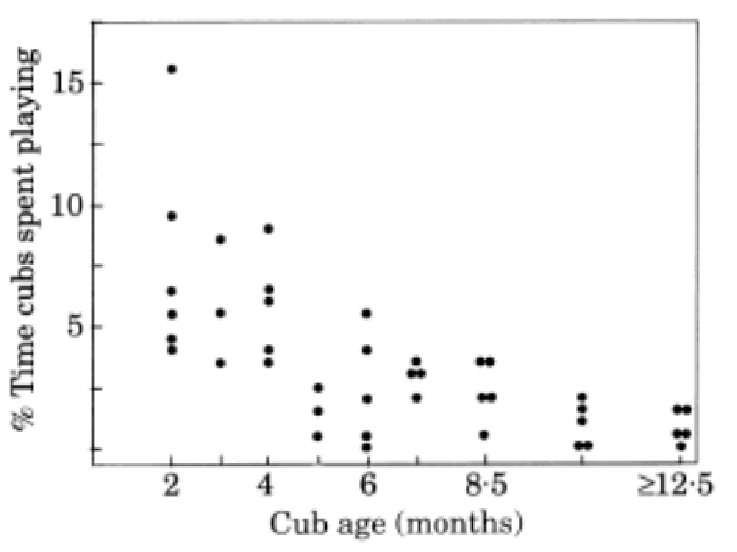
\includegraphics[width=83mm]{caroFig1edit.pdf}\\
	      b)\\
	      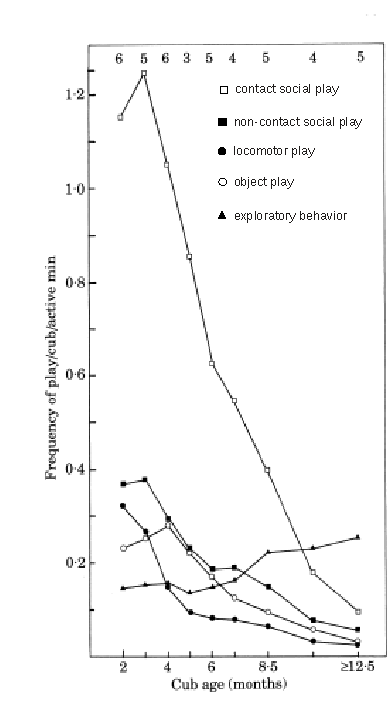
\includegraphics[width=80mm]{caroFig2edit.pdf}
	    \end{minipage}\hfill
	    \begin{minipage}[t]{0.43\linewidth}
	      $~$\\
	      a) The average percentage of time spent playing in 15 minute observations. 41 litters were observed. Each point represents an average for each litter. Total play decreases as cheetahs get older. 
	      \\\\\\\\
	      b) Running mean values of indicated play types. Number of litters from each age class shown across the top. Displayed play type changes with age, all types of social play decrease with age, while exploratory behavior increases with age. 
	    \end{minipage}
	  \end{center}
	\end{figure}

	
	%skill development line
	\begin{figure}[h!]
	\caption{A representation of the development of play behavior with respect to the model. In the terminal condition ($t=T$), $\phi(i)$ is defined based on the life history of the modeled organism for all time periods beyond $T$. The model is solved backwards in time to yield fitness values for every period of the model, $F(i,t)$, as well as play decisions for ever period of the model, $D^*(i,j,t)$.}
	\begin{center}
	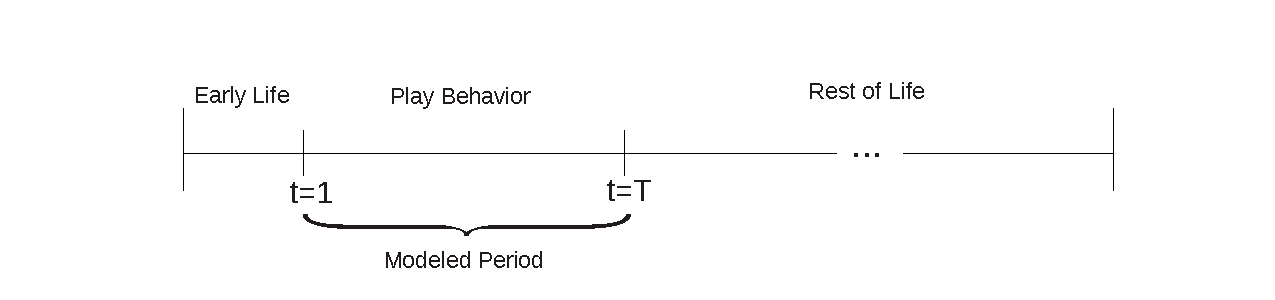
\includegraphics[width=170mm]{numberLineOfLife.pdf}
	\end{center}
	\label{sdf}
	\end{figure}
    
	%bell curve with Alpha Tau
	\begin{figure}[h]
	\caption{$\Delta S(i,j)$. The skill increment function showing several values of $\sigma$. $\Delta S(i,j)$ is plotted alongside the skill decrement $\alpha \tau$. Myopic focal individuals play with any play partner such that $i-j$ causes $\Delta S(i,j)>\alpha \tau$. Notice as $\sigma$ increases the range of potential play partners increases. For the optimal focal individual the play threshold lies some distance above $\alpha \tau$ based on the focal individuals skill and the amount of time remaining in the model.      }
	\begin{center}
	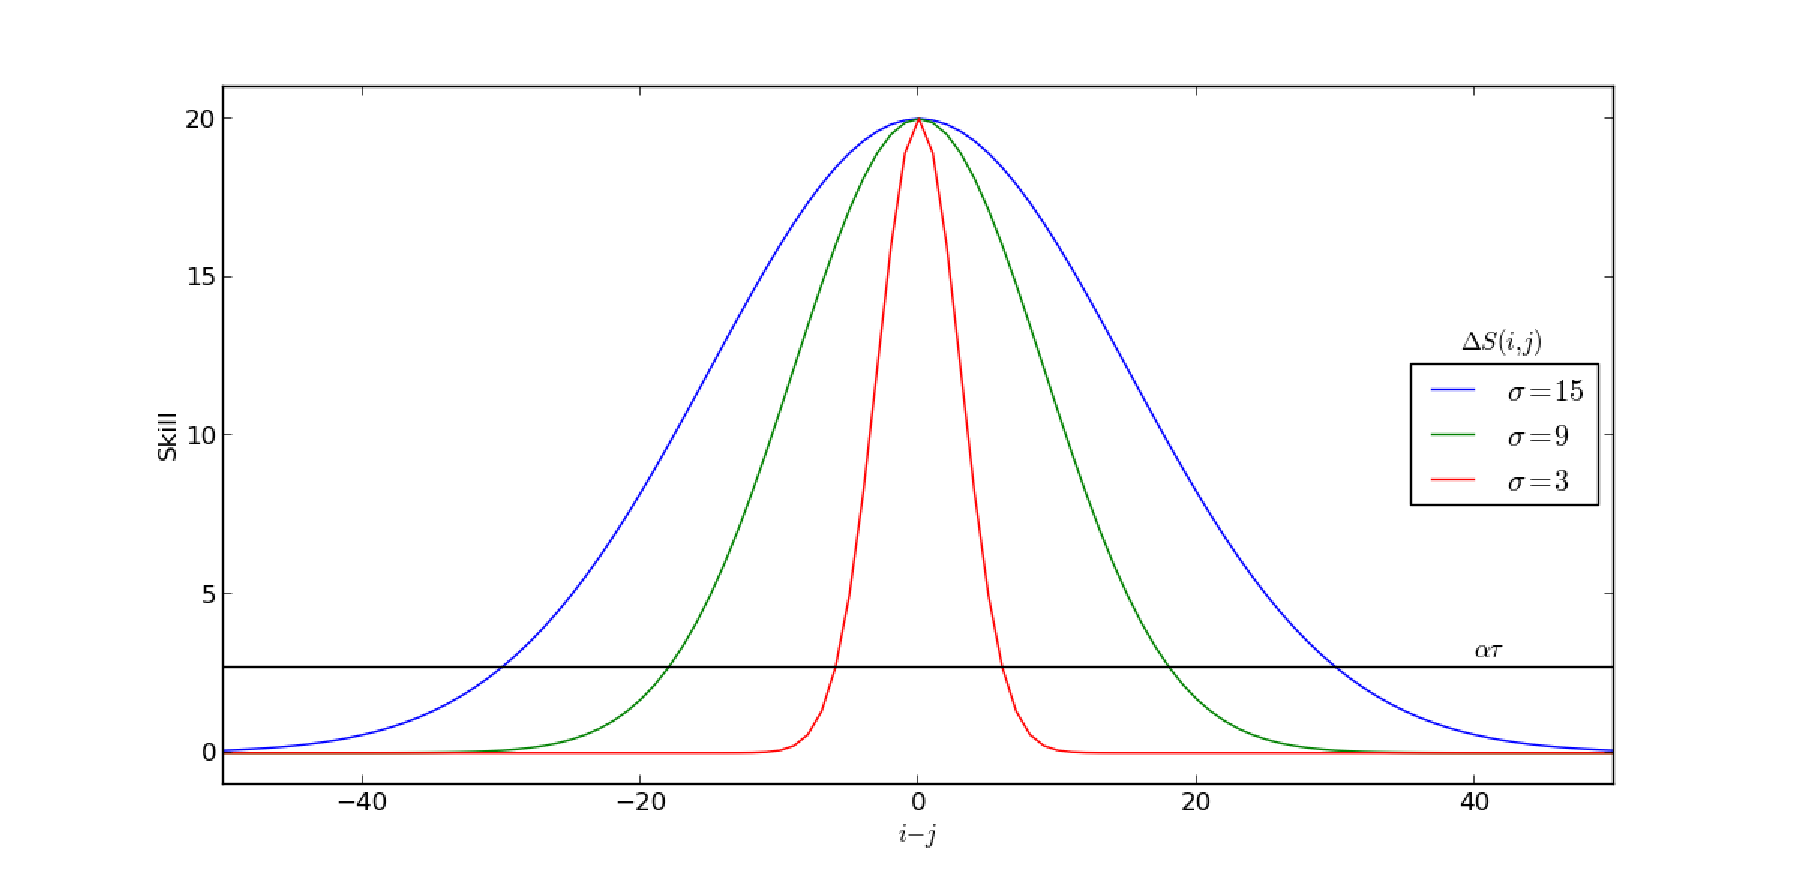
\includegraphics[width=160mm]{sdf.pdf}
	\end{center}
	\label{sdf}
	\end{figure}
	
	%future fitness
	\begin{figure}[h]
	\caption{$\phi(i)$. Three possible trajectories for $\phi(i)$. Notice the greater the steepness parameter $\gamma$ the more quickly and dramatically the organism matures once it reaches adolescence. }
	\begin{center}
	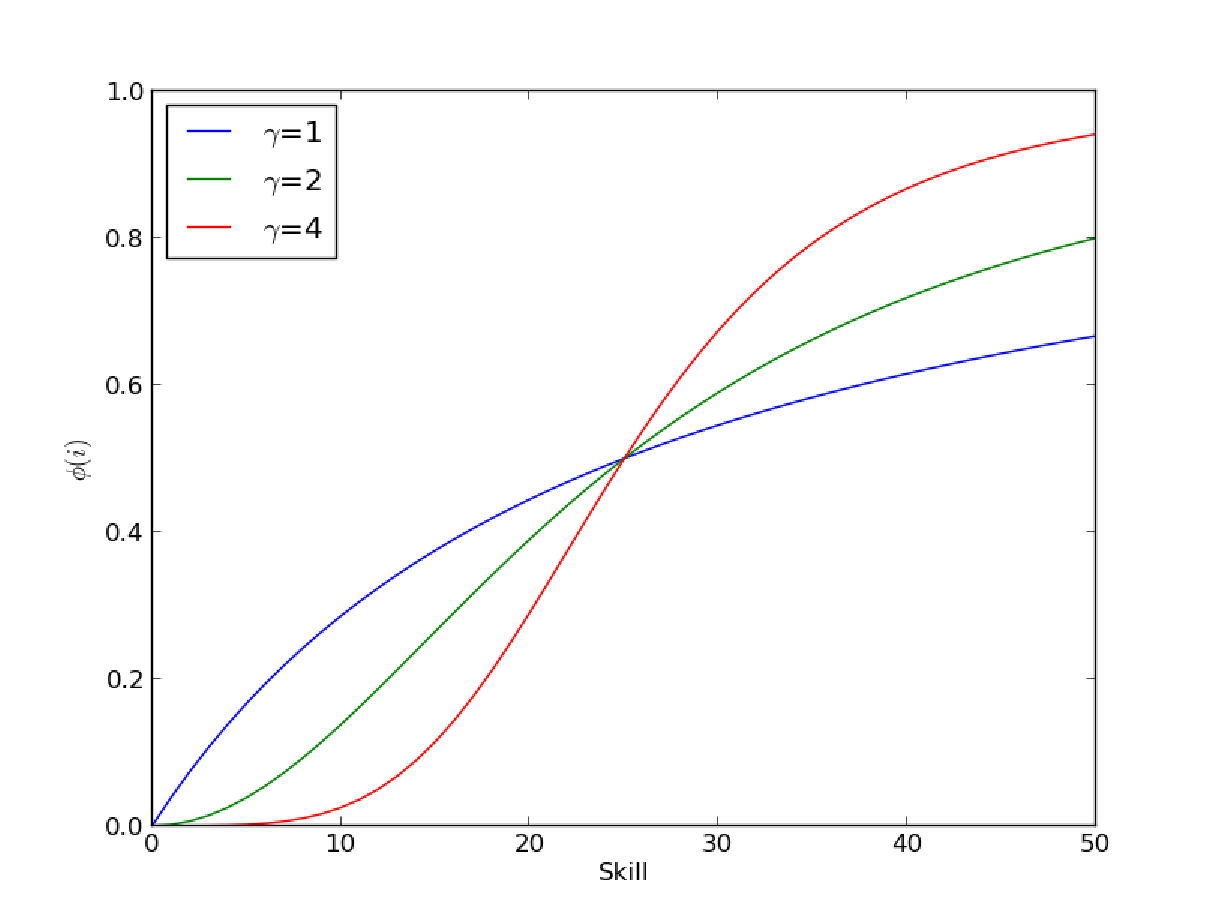
\includegraphics[width=160mm]{phi.pdf}
	\end{center}
	\label{phi}
	\end{figure}

	%heatmap
	\begin{figure}[h]
	\caption{$R(i,t)$. A grey scale representation of the focal individual play range as a function of both time and focal individual skill level. Dark cells are representative of focal individuals willing to play with play partners of many different skill levels, while light cells are representative of focal individuals with relatively small play ranges. In general as skill increases focal individual play range increases. Additionally as $t$ approaches $T$, in general, play range increases to the myopic condition, at $T-1$. However, a pocket of lower than expected play ranges does violate these general trends. This pocket occurs at relatively high values for $t$ and extends across all of the playing skill levels. This pocket is produced by truncating play events as $t$ approaches $T$. }%  .The complex patterns occurring at time periods just prior to $T-1$, at low skills, and time periods just prior to exiting, for high skills, are the effects of truncating of play events as $t$ approaches $T$.   }
	\begin{center}
	%\includegraphics[width=150mm]{playOpportunites.png}
	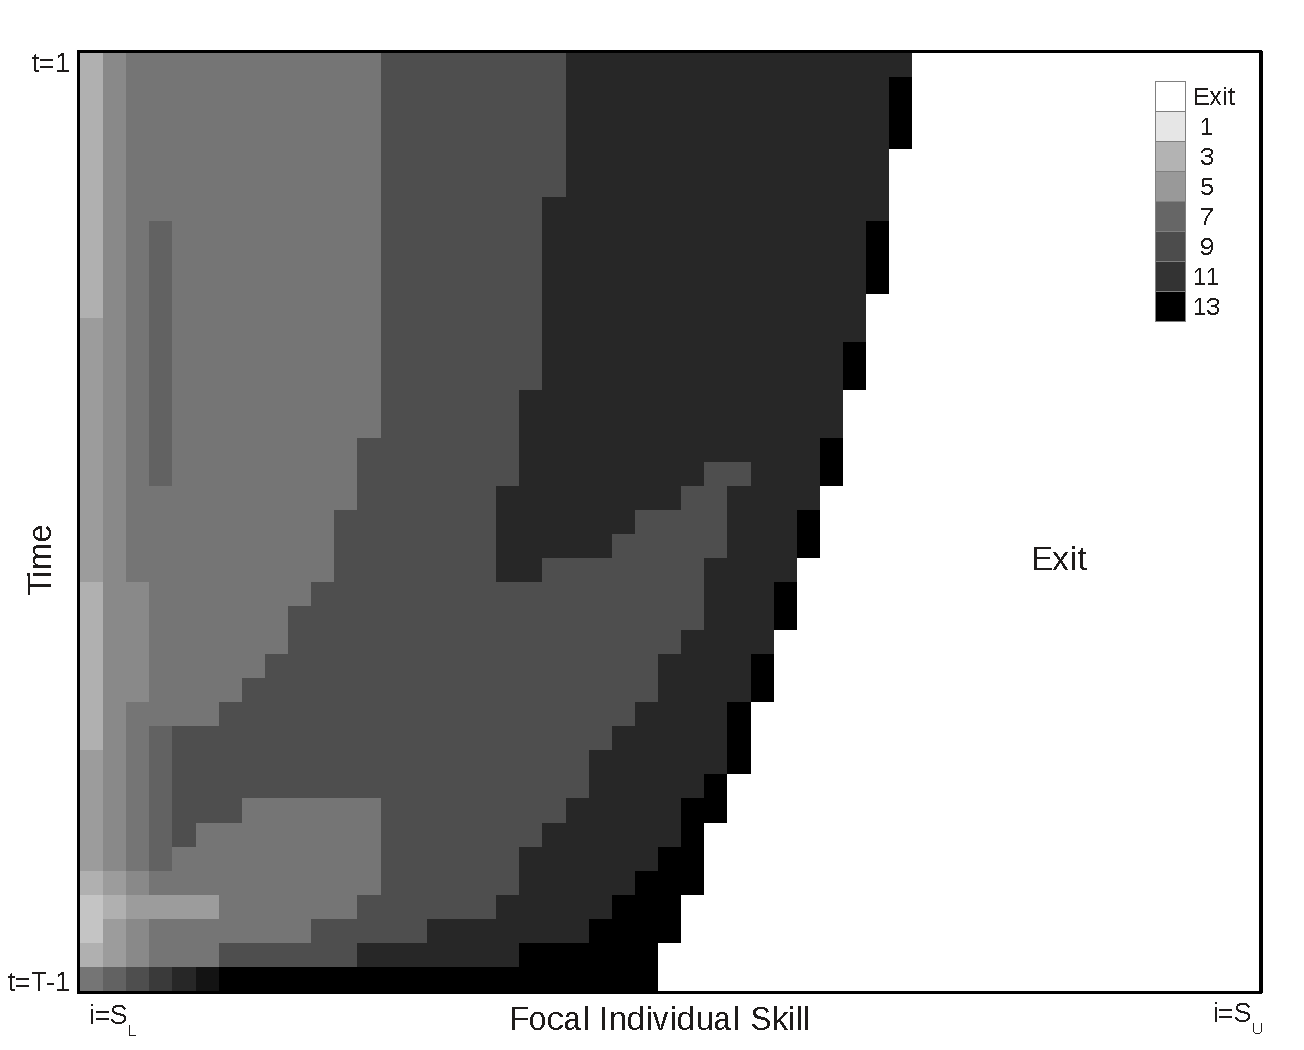
\includegraphics[width=170mm]{TplayHeat.pdf}
	%\label{map}
	%\caption{stay model}
	%\includegraphics[width=150mm]{playOpportunitesExit.png}\\
	%\includegraphics[width=150mm]{playOpportunitesExitBold.png}
	\end{center}
	\label{mapExit}
	\end{figure}

	%fitness at time
	\begin{figure}[h]
	\begin{center}
	\caption{$F(i,t)$. The focal individual fitness plotted against skill level. Each line is a single time period of the model. Three time periods of the model are plotted. Notice when many time periods remain in the model, fitness is relatively high for all skill levels, due to the prospect of gaining skill in the future. As the number of periods remaining in the model decreases, the fitness of low skill individuals decreases due to reduced prospect for the future. Additionally, the dotted vertical lines mark the skill at which $F(i,t)$ converges with $\phi(i)$. These dotted lines mark the skill at which the focal individual stops considering play behavior at the given time period of the model. Notice that with many time periods of the model remaining only very high skill individuals exit the model, and as the number of time periods remaining in the model decreases this exit skill decreases.  }
	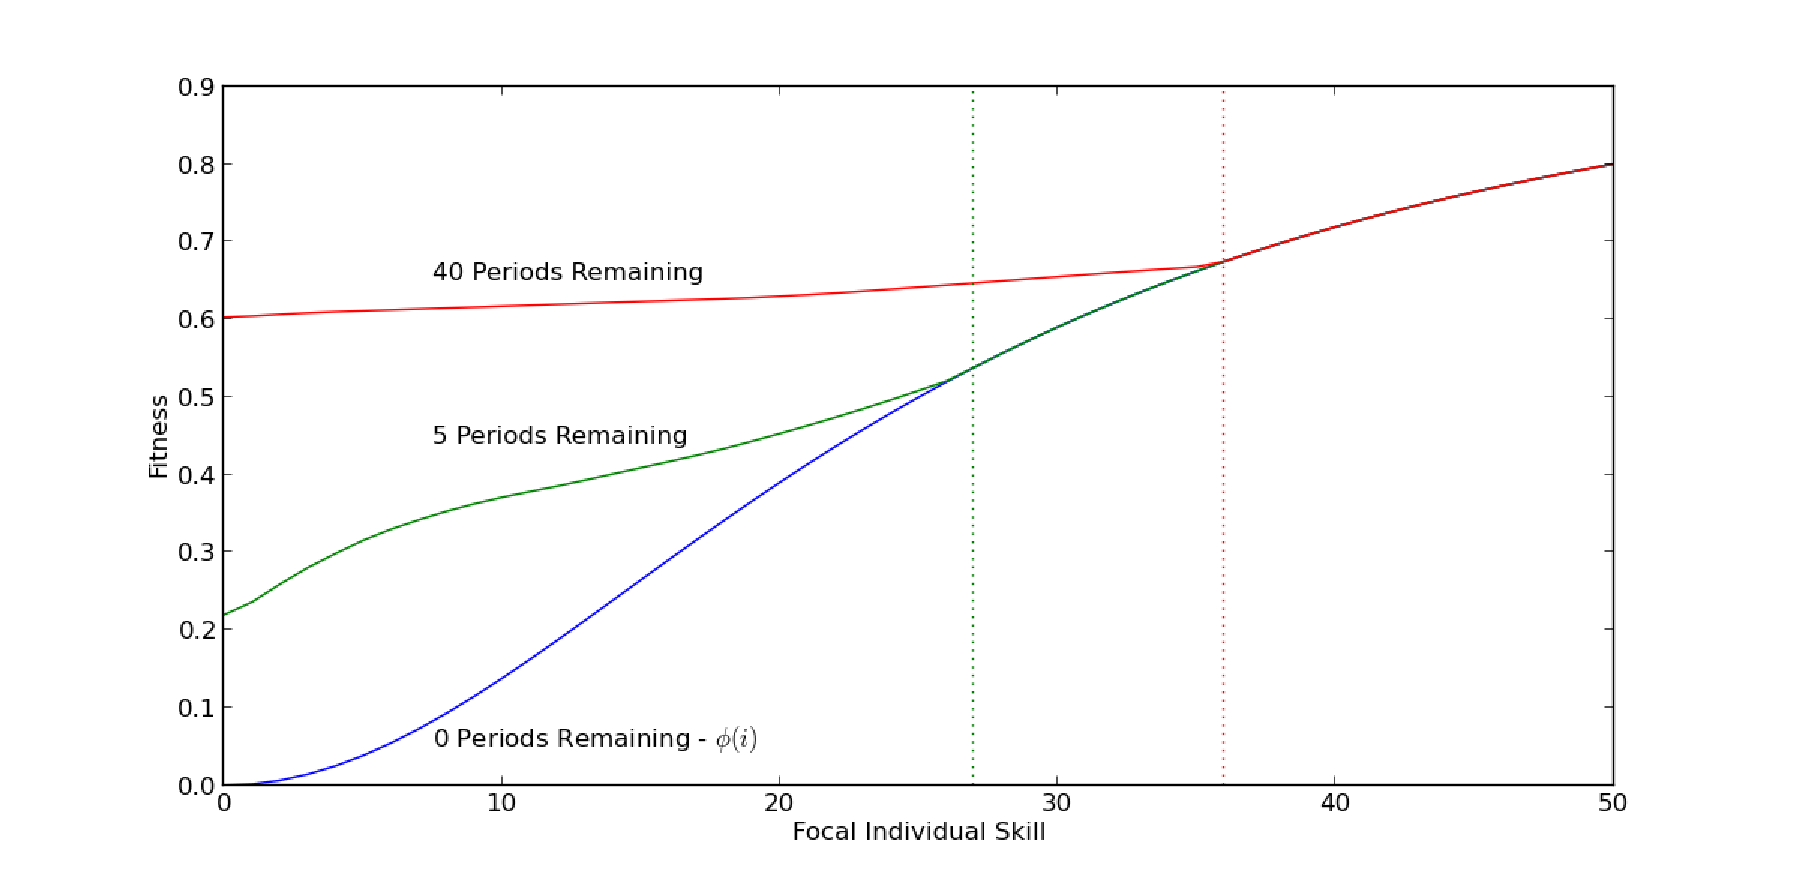
\includegraphics[width=160mm]{fitness.pdf}
	\end{center}
	\label{fit}
	\end{figure}
	
	\begin{figure}
	\caption{Final skill distribution of $k=250$ Monte Carlo simulated individuals. Each individuals starts the simulation with a uniform random skill level on the interval $[S_L,S_U]$. Each individual makes optimal decisions, based on $D^*(i,j,t)$, for 40 time periods. Notice the bimodal distribution of the final skills. }
	\begin{center}
	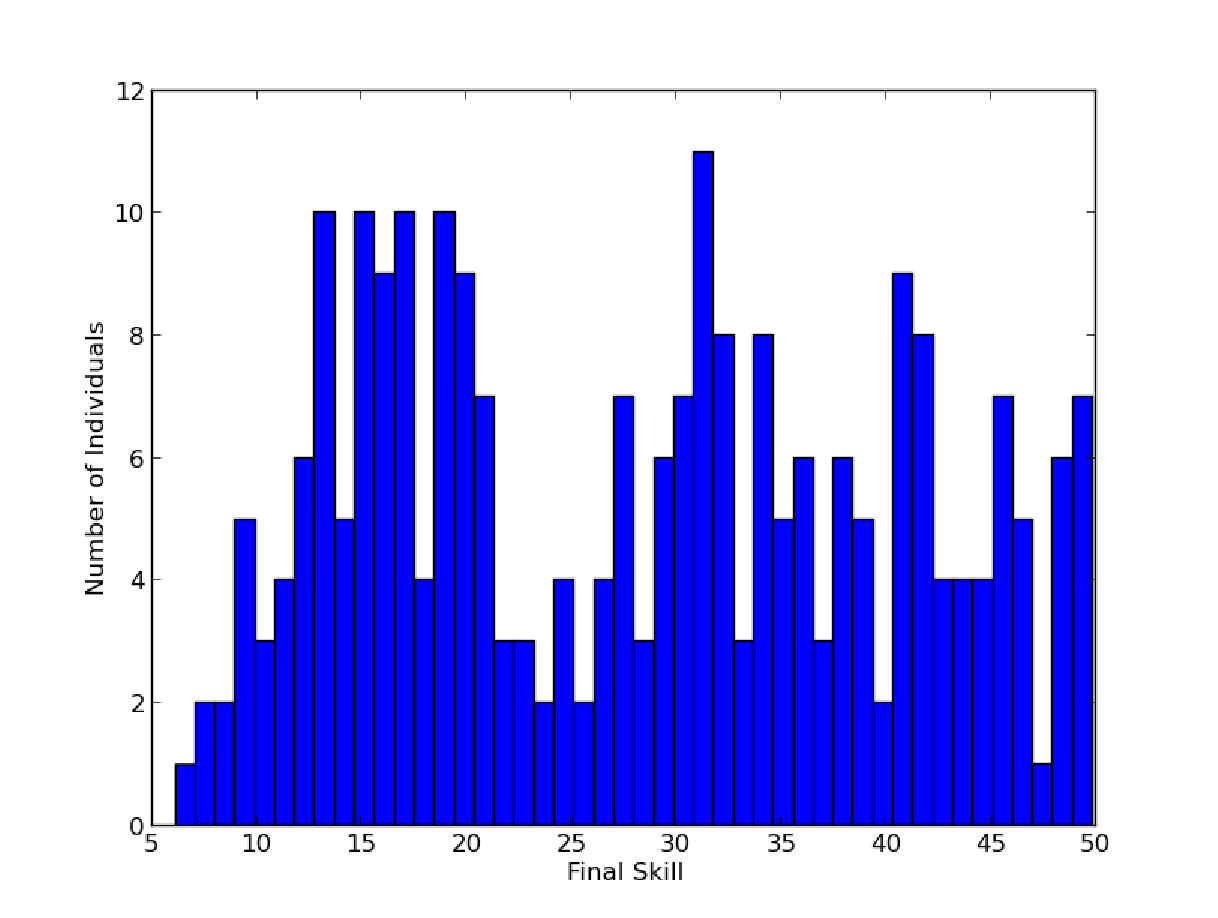
\includegraphics[width=150mm]{Fmcmc.pdf}
	\end{center}
	\label{Fmcmc}
	\end{figure}

	%scatter
	\begin{figure}[h]
	\caption{Final skill distribution of $k=250$ Monte Carlo simulated individuals plotted against the initial skill distribution. The red dotted line indicates the one-to-one relationship between initial and final skill. Individuals on the one-to-one line, in the region labeled ``Exit", enter the simulation with high enough skills to immediately exit play behavior. Notice for each initial skill below the initial exit skill, the final skill distributions are very similar, both to each other, and to the final skill distribution seen in Figure 7. }
	\begin{center}
	%\includegraphics[width=150mm]{mcmc.png}
	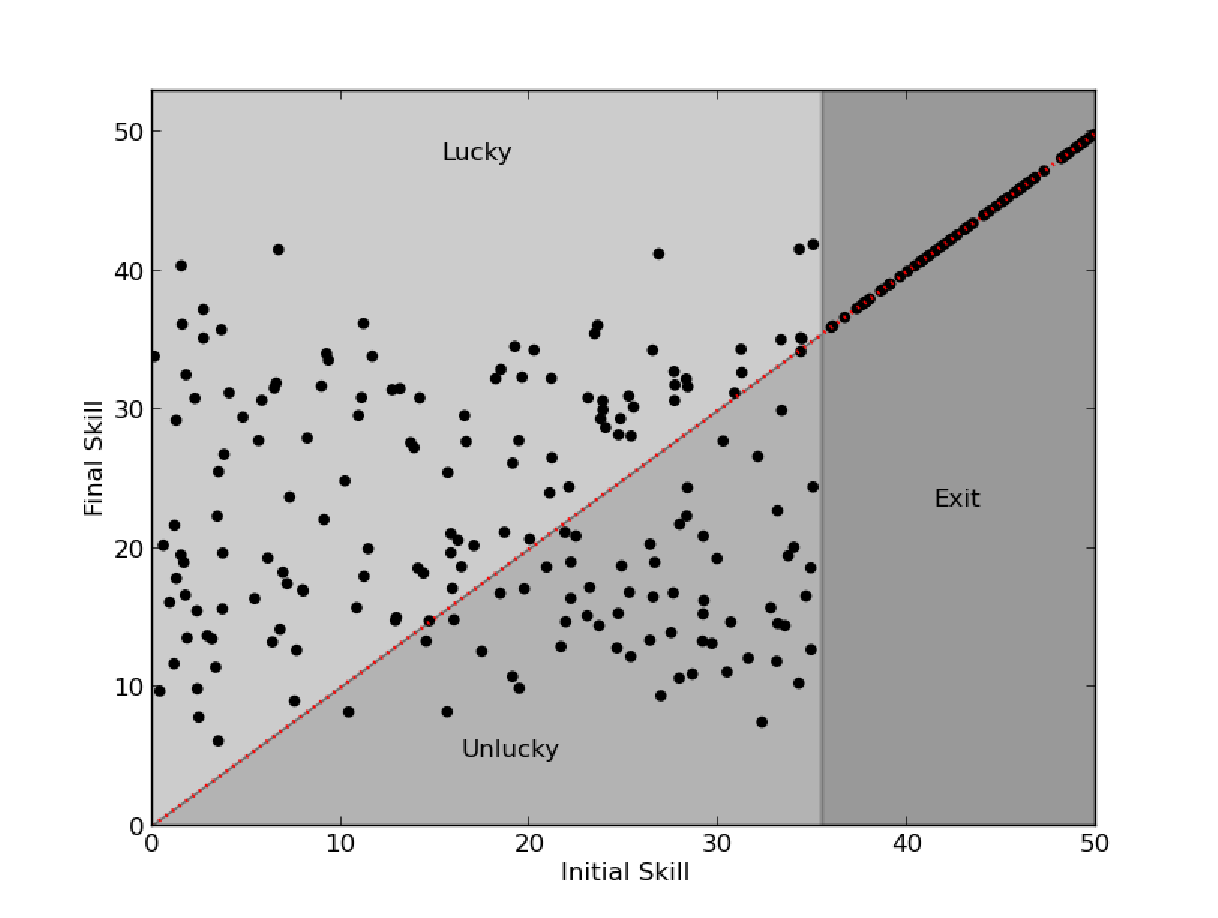
\includegraphics[width=150mm]{mcmc2.pdf}
	\end{center}
	\label{mcmc}
	\end{figure}

	
\end{document}